\section{Domain Case Studies}
\label{sec:cases}
In the previous section, the architectural foundations underlying the use of large language models (LLMs) in the context of human–machine interaction were introduced, encompassing text-based, audio-based, and vision–language modalities. 
This section builds on that foundation by reviewing selected studies from several safety-critical application domains; namely aerospace and remote sciences, emergency and environmental response, and industrial operations, with a focus on how LLM-based technologies are applied in human–machine interaction within these contexts.

\subsection{Aerospace and Remote Science}
Aerospace and remote science missions place humans in some of the most demanding HMI settings. 
Astronauts and mission operators work under high risk, limited communication, and long periods of isolation, while managing complex systems and strict safety procedures. 
In these conditions, interaction approaches that reduce cognitive effort, support decision-making, and offer context-aware assistance are especially valuable.
In this section, selected papers from this domain are analyzed and discussed.

\subsubsection{Conversational User Interfaces to Support Astronauts \cite{freitas2021conversational}}

This paper uses a Wizard of Oz (WoZ) study\footnote{A Wizard of Oz study is an experimental method in which users interact with an apparently autonomous system whose behavior is secretly controlled by a human operator, which enables the study of interaction patterns before full system implementation.\cite{dahlback1993wizard}} to investigate how astronauts would realistically interact with a conversational user interface (CUI) inside an extraterrestrial habitat before such a system technically exists.
It investigates how CUIs can support astronauts living and working in extraterrestrial habitats (Moon/Mars), where isolation, confinement, delayed communication with Earth, and psychological stress are major challenges.

To address these differing interaction requirements, the authors designed two complementary CUIs: CASSIOPEIA, which provides task-oriented, mission-critical assistance for scientific operations, and PEGASUS, which functions as an emotionally expressive personal companion to support crew well-being.

While designing the conversational user interfaces (CUIs), the authors identified four key design guidelines:

\begin{itemize}
    \item \textbf{Support both mission-critical and non-mission-critical interactions}, ensuring reliable task execution while also accommodating informal and supportive exchanges.
    \item \textbf{Design for frequent and prolonged use}, accounting for long-duration missions and sustained human--AI interaction without inducing cognitive fatigue.
    \item \textbf{Enable multimodal and bidirectional interaction}, allowing users to interact with the system through complementary input and output modalities such as text, speech, and visual feedback.
    \item \textbf{Design the CUI as a team member}, positioning the interface as an active collaborator that supports coordination, shared situational awareness, and trust within the crew.
\end{itemize}

\textbf{Method}

To derive requirements for conversational user interfaces in extraterrestrial habitats, the authors conducted a week-long Wizard-of-Oz study inside the MaMBA Moon/Mars habitat laboratory module at ZARM. 
Four experienced scientists carried out real biological, geological, and materials science experiments while interacting with a simulated CUI operated by a human wizard via a Raspberry Pi–based voice interface. 
All interactions were logged, video-recorded, transcribed, and qualitatively coded, revealing frequent use of both mission-critical and non-mission-related interactions. 
Based on these findings, the authors derived four design guidelines emphasizing support for mission and non-mission tasks, intensive long-term use, multimodal and bidirectional interaction, and the treatment of the CUI as a team member. 
Guided by these principles, the two CUIs introduced earlier were implemented.
These systems were evaluated in two controlled user studies within the habitat: one comparing voice-only versus voice-plus-GUI interaction for task efficiency, and another comparing emotionally characterized versus neutral CUIs to assess emotional engagement, stress, and workload using standardized questionnaires and interviews.

\begin{figure}[H]
    \centering
    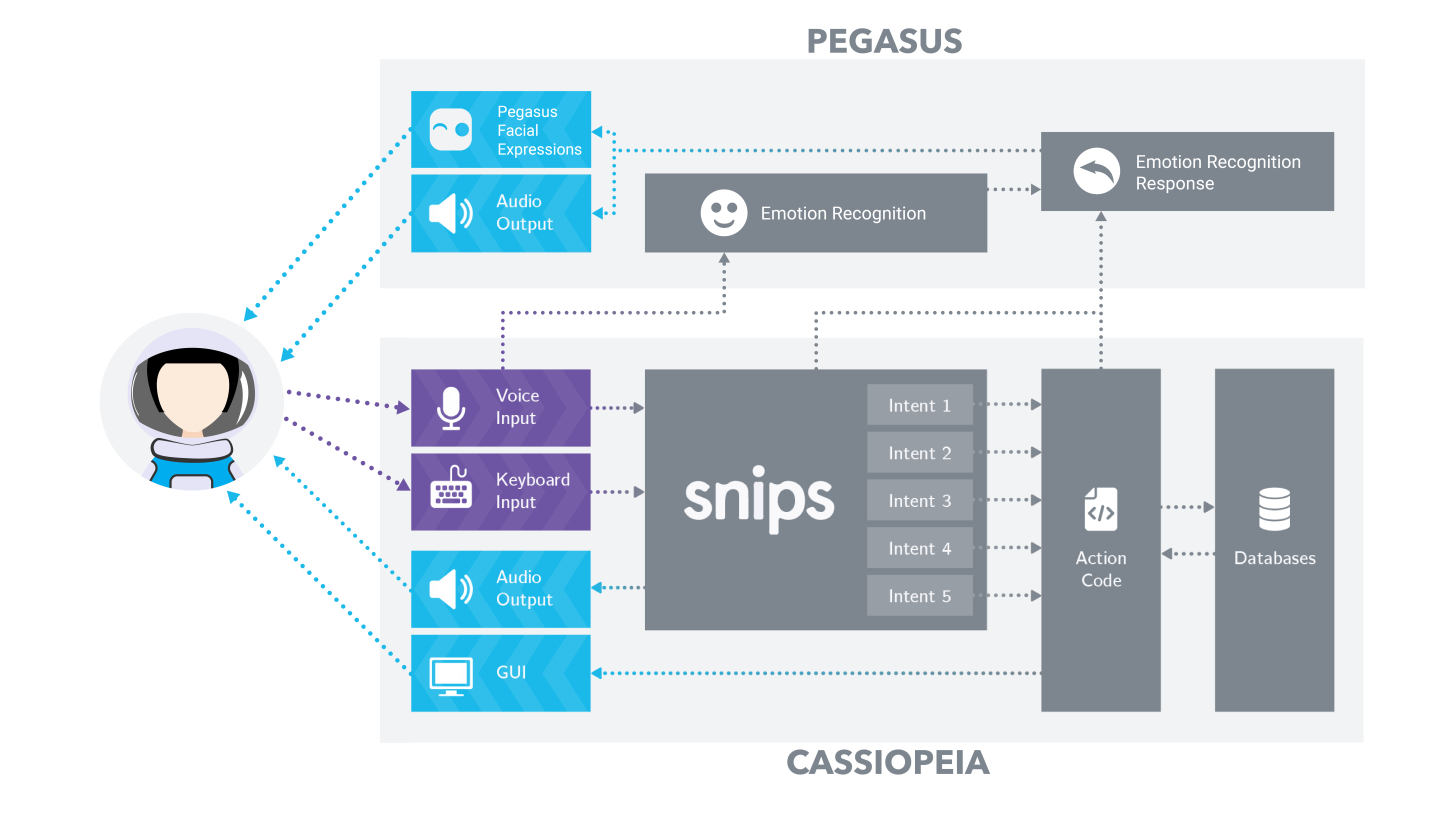
\includegraphics[width=0.8\linewidth]{bilder/Cassiopei/Pegasus.png}
    \caption{Overview of the PEGASUS and CASSIOPEI companion CUIs: multimodal astronaut inputs are parsed through intent recognition, emotional context, and action code to provide both operational and affective support.\cite{freitas2021conversational}}
    \label{fig:pegasus_architecture}
\end{figure}

\textbf{Result}

The study shows that CUI can meaningfully support astronauts in isolated extraterrestrial habitats by improving both task performance and user experience. 
Results indicate that multimodal CUIs combining voice and graphical interfaces enable significantly more efficient task completion than voice-only CUIs, while perceived usability remains comparable. 
Emotionally characterized CUIs increase user excitement and engagement, and stronger emotional connection and perceived sympathy toward the system are associated with lower reported stress levels, although individual responses vary and overall task workload does not differ significantly. 
Overall, the findings suggest that well-designed CUIs can enhance operational efficiency and psychological well-being in long-duration space missions, provided that emotional interaction and interface modality are carefully adapted to user needs.

\textbf{Analysis}

Freitas et.al. propose a framework for the design and development of conversational user interfaces for space missions in this paper. 
Although the study employs a Wizard-of-Oz setup in which a human operator simulates the AI system, the results provide a convincing proof of concept demonstrating that the development of such assistants is both feasible and worthwhile. 
Building on the proposed framework, a fully autonomous implementation that integrates real-time speech-to-speech models, retrieval-augmented generation, and tool-calling mechanisms represents a promising direction for future research. 
Such an approach could combine several aspects discussed in the background section of this paper to realize an agentic conversational system capable of supporting astronauts in safety-critical and isolated mission environments.


\subsubsection{AI Assistants for Spaceflight Procedures: Combining Generative
Pre-Trained Transformer and Retrieval-Augmented Generation on
Knowledge Graphs With Augmented Reality Cues \cite{bensch2024aiassistants}}

In this paper Bensch et.al. intoduce an intelligent personal assistant (IPA) they named CORE (Checklist Organizer for Research and Exploration).
CORE is designed to support astronauts during procedural tasks on the ISS, Lunar Gateway, and future deep-space missions.
It combines Large Language Models (GPTs) with Retrieval-Augmented Generation (RAG), Knowledge Graphs (KGs), and Augmented Reality (AR) to achieve its tasks.
\\

\textbf{Method}

The authors validate CORE through qualitative, prototype-based functional testing rather than formal benchmarking. 
Ten publicly available ISS procedures were indexed into a vector database and linked with metadata and images via a knowledge graph, forming the basis of a retrieval-augmented generation (RAG) pipeline built on GPT-4. 
Spoken user queries were transcribed using Whisper, enriched with retrieved procedure content, and used to generate constrained responses. 
Validation was performed using example queries to verify that CORE returned the correct procedure steps verbatim and triggered associated visual cues, while rejecting non-procedure-related questions. 
In addition to this functional validation, offline availability is addressed as a system design consideration: the authors argue that recent advances in open-source large language models, together with optimization techniques such as low-rank adaptation and quantization, make fully offline deployment of the proposed architecture feasible for future missions. 
However, this offline capability is not empirically evaluated in the present work. 
No quantitative performance metrics or user studies are reported; a controlled evaluation at the European Astronaut Centre is explicitly deferred to future work.\\

\textbf{Result}

The authors demonstrate that the CORE prototype can correctly retrieve and present procedural information using a Retrieval-Augmented Generation architecture. 
In their experiments, CORE successfully returned exact, verbatim procedure steps in response to user queries, including the correct step numbering and associated visual references when available. 
The system was able to answer both step-specific questions (e.g., requesting a particular step in a CPR procedure) and metadata-related queries (such as the last update date of a procedure), reformulating retrieved graph data into coherent natural-language responses. 
Importantly, CORE consistently rejected questions unrelated to the indexed procedures, enforcing strict domain boundaries and reducing the risk of hallucinated or unsafe responses. 
These results indicate that the proposed combination of GPT, RAG, and knowledge graphs can support reliable, constrained procedural assistance. 
However, the reported results are illustrative and qualitative, and no quantitative performance metrics, comparative baselines, or user-study outcomes are provided.
\\

\textbf{Analysis}

Bensch et al. demonstrate that the development of an AI-based procedural assistant for space missions is technically feasible. 
They adopt a modular speech-to-text, language model, and text-to-speech (STT–LLM–TTS) pipeline, which enables seamless integration with a vector database through Retrieval-Augmented Generation (RAG). 
According to the authors, this architectural choice allows the system to retrieve reliable, procedure-specific information while reducing the risk of hallucinated responses. 
However, the paper lacks an in-depth evaluation of the system’s capabilities; the limited number of illustrative prompt–response examples is insufficient to establish the robustness or generalizability of the approach. 
Furthermore, no user study is conducted to assess usability, user acceptance, or cognitive workload during interaction. 
As the system relies on a pipeline-based interaction model rather than an end-to-end speech-to-speech approach, response latency may be higher, potentially reducing conversational naturalness and introducing an “uncanny valley” effect. 
Despite these limitations, the authors’ emphasis on offline-capable deployment represents a particularly important contribution, as reliance on cloud-based models is impractical in space environments due to communication delays and outages. 
This aspect highlights promising directions for future research, including the development of onboard data processing infrastructure capable of locally hosting large language models for autonomous space operations.

\subsubsection{LLM-Based Autonomous Agent for Aerospace Wire Harnessing \cite{wang2026llmharnessing}}
In this paper, Wang et al. introduce an agent-based framework for human–robot collaboration (HRC) and validate it through a high-precision aerospace wire harnessing assembly use case. 
Building on existing tool-calling and agentic reasoning paradigms discussed in Section 2, the framework extends these approaches by incorporating long-term memory mechanisms, implemented via vector database embeddings, to support contextual understanding, and iterative task execution.


The proposed system is an agent-based human–robot collaboration (HRC) framework in which a large language model (LLM) is embedded into a robotic system as an autonomous decision-making agent. 
Rather than treating the LLM as a passive instruction parser, the framework elevates it to an agentic role, capable of reasoning, planning, executing actions through tools, observing outcomes, and adapting behavior over time. 
Human operators interact with the system primarily through natural language instructions, provided in text or speech form, while the robot executes physical actions and provides implicit feedback through its movements and task outcomes; continuous collaboration is achieved by allowing the human to issue incremental or corrective instructions during execution, which are interpreted by the agent using contextual memory and integrated into subsequent planning steps.
An overview of the individual modules is provided below.

\begin{itemize}
    \item \textbf{Configuration Module:} 
    Defines the agent’s role, goals, behavioral constraints, available tools, and prompt structure, ensuring that the LLM operates as a task-oriented autonomous agent rather than a conversational chatbot.

    \item \textbf{Task Planning Module:} 
    Uses an unmodified LLM within a Reason--Act chain-of-thought loop to interpret human instructions, decompose complex tasks, and determine which actions and tools should be invoked at each step.

    \item \textbf{Task Execution Module:} 
    Executes the planned actions by invoking encapsulated tools for perception, coordinate transformation, and robot control, and returns execution outcomes to the agent as observations.

    \item \textbf{Memory Module:} 
    Maintains short-term contextual memory and long-term vector-embedded summaries of past interactions to support continuous, context-aware reasoning across multiple tasks.
\end{itemize}

\begin{figure}[H]
    \centering
    
\includegraphics[width=0.7\linewidth]{\detokenize{bilder/HUman Robot CCollab.png}}
    \caption{LLM-driven human--robot collaboration workflow showing how instructions propagate through prompting, memory, tool calls, execution, and feedback loops to support industrial assembly tasks. \cite{wang2026llmharnessing}}
    \label{fig:hrc_workflow}
\end{figure}

\textbf{Method}

The proposed HRC agent is validated experimentally using a real-world human–robot collaborative assembly setup based on a UR5 collaborative robot equipped with a depth camera and vision system. 
Validation is conducted progressively across three capability levels: perception, task planning, and task execution. First, the agent’s sensing ability is evaluated using a Target Recognition Success Rate (TRR), which measures the correctness of object detection and spatial localization for tools, connectors, cables, and assembly ports under repeated trials, including dense connector arrays handled via a grid-matching recovery method. 
Second, the cognitive task-planning capability is assessed independently of robot execution by providing natural-language instructions and evaluating whether the agent’s chain-of-thought reasoning produces correct and executable action sequences, quantified using the Task Planning Success Rate (TPR) and benchmarked against state-of-the-art standalone LLMs under identical tool constraints. 
Third, full end-to-end task execution is validated by deploying the planned action sequences on the physical robot and measuring the Task Execution Success Rate (TER), requiring all subtasks to be successfully completed in real assembly scenarios. 
Each task is repeated multiple times to assess robustness, and additional experiments demonstrate the agent’s generalizability to previously unseen wire assembly tasks, thereby validating perception, reasoning, and execution capabilities in an integrated industrial setting
\\

\textbf{Result}

The proposed HRC agent demonstrates consistently high success rates across perception, task planning, and execution in real aerospace wire harnessing assembly experiments, with most tasks achieving 9–10 successful trials out of 10 repetitions. 
In task planning, the agent substantially outperforms standalone state-of-the-art LLMs, which frequently fail to generate correct and executable action sequences for domain-specific assembly tasks. 
Overall, the results indicate that the agent-based LLM framework enables robust and reliable human–robot collaboration in complex industrial environments
\\

\textbf{Analysis}

The paper presents a technically solid and credible system, with results that are convincing within the tested industrial context, particularly because validation is performed on a real robotic setup rather than in simulation. 
Reported success rates (mostly 9–10 out of 10 trials) indicate robust performance, and comparisons with standalone LLMs support the claim that the agent-based architecture is the key contributor. 
However, the evaluation is limited in scope, lacks statistical analysis and ablation studies, and does not include human-centered metrics, so the results should be viewed as a strong proof of concept rather than evidence of broad generalizability.

Moreover, the system does not employ retrieval-augmented generation and instead relies on the language model’s internal memory for context understanding, which limits access to explicit domain knowledge. 
Integrating a RAG mechanism to retrieve subject-specific assembly or process information would be a natural improvement to enhance robustness and scalability.

\subsection{Emergency and Environmental Response}

\subsection{Industrial Operations}

Industrial operations are an early proving ground for LLM-enabled human--robot collaboration workflows that can translate operator intent into contextual tool use, perception, and execution. Figure~\ref{fig:hrc_workflow} summarizes one such architecture integrating prompt templates, multimodal memory, tool libraries, and action monitoring loops tailored for collaborative assembly tasks.

